%% Status: 2015-12-30 Some parts collected from wiki.
%% TODO: Describe StellariumScope plugin

\chapter{Stellarium at the Telescope}
\label{ch:atTheTelescope}

Two plugins are bundled with Stellarium which are designed to be used
at the telescope: Oculars, which provides field of view hints for
telescopes, oculars and sensors, and TelescopeControl, which allows
you to send GOTO commands to many motorized telescopes. Other goto
telescopes are supported by an external plugin which you must install
separately: StellariumScope (section~\ref{sec:plugins:StellariumScope}). 

\section{Oculars Plugin}
\label{sec:plugins:Oculars}

TODO

\section{TelescopeControl Plugin}
\label{sec:plugins:TelescopeControl}

TODO

\section{StellariumScope plugin}
\label{sec:plugins:StellariumScope}
StellariumScope is a free add-on that enables you to control your telescope with Stellarium. 

\paragraph{Features}
\begin{itemize}
\item Provides an interface between Stellarium and the ASCOM telescope drivers.
\item Provides the ability to both ``Sync'' and ``Slew'' the
  telescope. It's also possible to issue a stop/cancel command from
  Stellarium.
\item You can easily host Stellarium on one computer linked to another
  control computer that hosts the telescope driver.
\item The installation program will automatically install the
  documentation, but the link to the documentation is provided
  here\footnote{WHERE?} so you can read it before installation.
\item There are earlier releases still available on the downloads page on
  Welsh Dragon Computing site.
\end{itemize}

The original StellariumScope program was designed and implemented by
Scott of ByteArts and is still available for
download\footnote{\url{http://www.bytearts.com/stellarium/}}. If you
have difficulties with the releases available on the Welsh Dragon
Computing
site\footnote{\url{http://welshdragoncomputing.ca/x/index.php/home/stellariumscope/about-stellariumscope}},
you may want to consider using the original version.

\begin{figure}[h]
\begin{center}
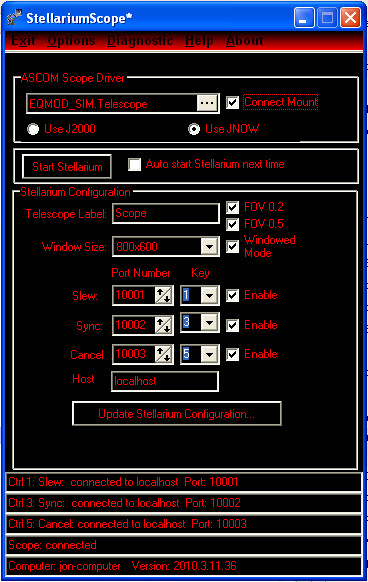
\includegraphics{StellariumScopeFullWindow.jpg}
\end{center}
\label{fig:StellariumScopeFullWindow}
\caption{StellariumScope interface}
\end{figure}

Figure~\ref{fig:StellariumScopeFullWindow} shows the interface and
some of the options.  Use this application (like all software that
controls your mount) with supervision of your mount's movements.

\subsection{Configure StellariumScope}
\label{sec:plugins:StellariumScope:configure}
TODO...
\subsection{Download StellariumScope}
TODO...


\section{Observability Plugin}
\label{sec:plugins.Observability}

TODO...


%%% Local Variables: 
%%% mode: latex
%%% TeX-master: "guide"
%%% End: 

